\section{AES}
The Advanced Encryption Standard (AES) is a widespread symmetric cryptosystem. AES is primarily used as a block cipher, which has openly exploitable parallelism by encrypting multiple blocks at once. Thus we saw AES as a prime candidate to optimize with hardware for large amounts of data. The AES implementation was based off of the NIST documentation\footnote{NIST guide to AES: \url{https://nvlpubs.nist.gov/nistpubs/FIPS/NIST.FIPS.197.pdf}.} on AES as well as the github library "tiny-AES-c"\footnote{Embedded optimized tiny-AES-c library: \url{https://github.com/kokke/tiny-AES-c}.}.

\subsection{Techniques}
% This section should provide a detailed description of the applications, algorithms, or
% hardware architectures realized in this project. Think critically about the important items to mention
% in order for the reader to understand how your design works without having to look into any code.
% For example, what are the inputs and outputs of the application (or architecture), what are the major
% steps (or modules), and what does each step (or module) achieve? It would be useful to include
% small examples, block diagrams, mathematical formulas, and other visualizations to help explain your
% techniques. Do not include detailed information about your source code as your report should be at a
% high level.
The AES algorithm consists of a number of rounds operating on a 4x4 byte matrix state to encrypt a 16-byte buffer input using a key. The key can be either 128, 192, or 256 bits wide. The larger the key, the more rounds are run on the state. Each round consists of four main operations called "AddRoundKey", "SubBytes", "ShiftRows", and "MixColumns".
Initially, the user-provided key is expanded a key schedule, called the "RoundKey".
During "AddRoundKey", a portion of the "RoundKey" the state is updated by an XOR with a portion of the "RoundKey".
"SubBytes" is a one-to-one substitution of each byte value in the state using the Rijndael S-box. \footnote{The S-box is constructed using finite field arithmetic, which is beyond the scope of this paper.}
"ShiftRows" is a rotation of rows in the matrix by differing offsets.
Lastly, "MixColumns" operates on the columns of the state, performing some matrix multiplication with each column, but also additional Galois Field-related computations that are beyond the scope of this paper.

The algorithm described above encrypts a single input block. In order to exploit the high-level parallelism, we want to encrypt multiple input blocks at once.
There are many standard encryption modes which specify how a multi-block message should be encrypted.
Electronic Cookbook mode (ECB) encrypts each block individually, but is very insecure as identical blocks in the input message manifest as identical blocks in the output message.
Cipher Block Chaining (CBC) XORs each block's plaintext with the encrypted prior block, forming a ``chain''. It is secure, but prevents parallel encryption, since each block depends on the prior block.
Counter mode (CTR) solves this problem. It starts with a random \emph{Initialization Vector} (IV, also known as a nonce). Block $n$ is encrypted by XORing it with the encrypted value $IV + n$.
This eliminates the dependencies between blocks, and still provides a secure cipher.
This allows us to pipeline the encryption easily as each value being encrypted is one plus the previous value.
Figure \ref{fig:aesctr} shows with a diagram how AES CTR works, taking in 16-byte blocks and encrypting them with AES.

\begin{figure}[h]
\centering
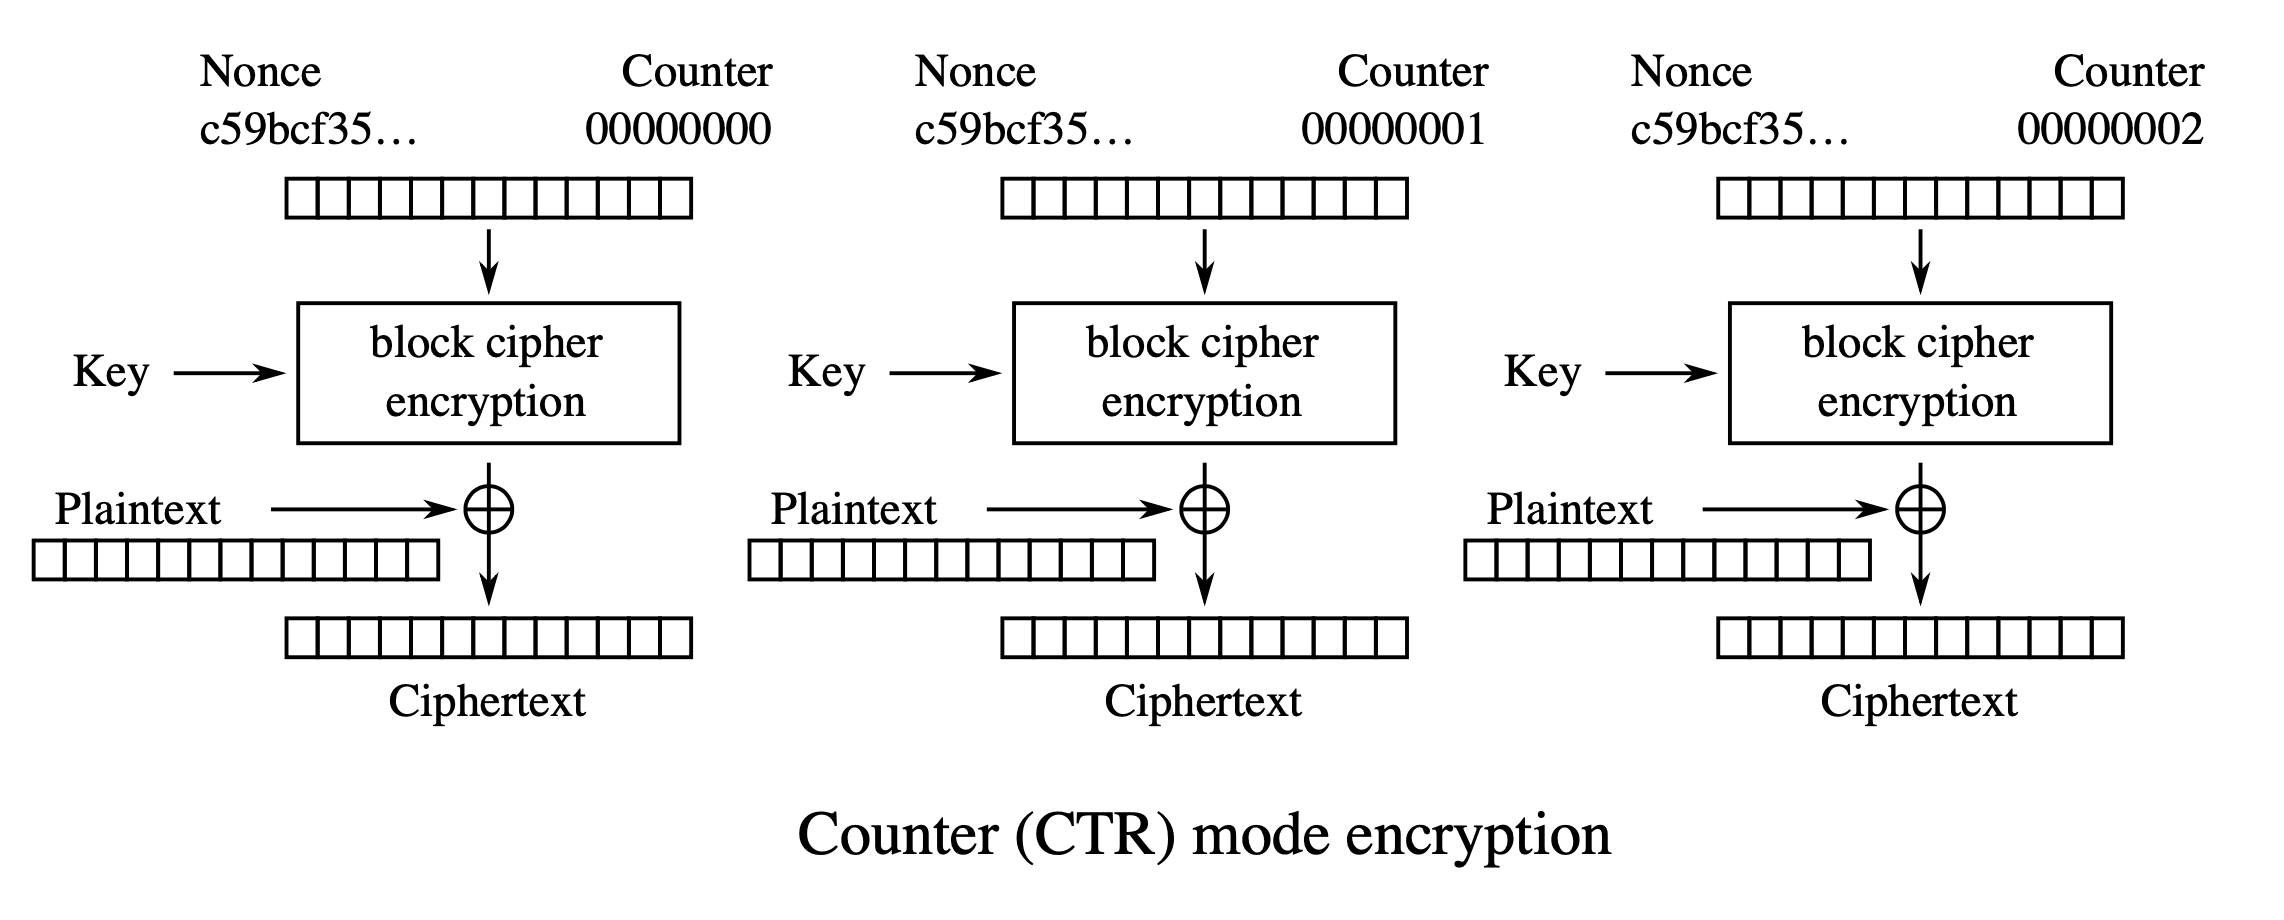
\includegraphics[width=0.5\textwidth]{aesctr}
\caption{AES CTR diagram.}
\label{fig:aesctr}
\end{figure}

\subsection{Implementation}
% This section describe how you implemented your designs. For example, what
% programming languages did you use? Did you take advantage of any third-party libraries? Is your
% implementation purely software, purely hardware, or a mix of both? Which software and/or hardware
% blocks are included in your design, and what hardware device (if any) did you target? In most cases, it
% would be helpful to include block diagrams of your implementation illustrating the flow of data through
% your design, the interconnection between different blocks, and whether each block is implemented
% in software or hardware. As in the previous section, providing meaningful visualizations would help
% the reader better appreciate your work. Please also include one or two interesting aspects of your
% implementation, especially any specific implementation strategies necessary for creating a functionally
% correct design with good performance.
Our optimized hardware synthesizable version was built using C++ and the Vivado "ap_int" library.
Normally AES is implemented by taking a 16-byte array and converting that into a 4x4 byte matrix as the state, storing the bytes as in Figure \ref{fig:aesstate}.
We packed the 16-byte block into one 128-bit number. The key is also stored as an X-bit number, where the X is determined by the key length.
The RoundKey is packed into an array of 128-bit numbers, one for each of the 10 rounds.
This makes the "AddRoundKey" function a single XOR with the current round's key schedule.
The other functions (except "ShiftRows"), contain loops to loop over each byte or each column.
These we completely unroll, as they can all be done in parallel, and it actually reduces area because indexing into the large "ap_uint"s variably was more expensive than direct wires connected to the bits of the state.
"ShiftRows" was already just a bunch of wire rearrangements and required no optimization.
The four main functions had 0 or 1 cycle latencies, the 1 cycle for indexing into the Sbox or the RoundKey arrays.
Ideally we could fully partition those, and reduce those latencies to just combinational logic, but this took too much area.

\begin{figure}[h]
\centering
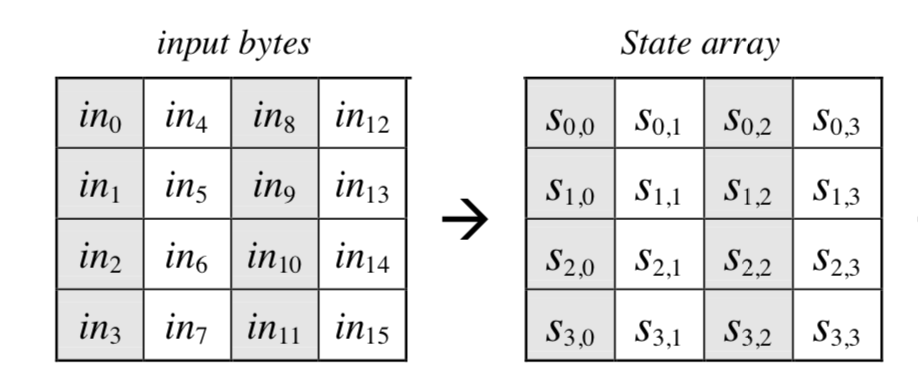
\includegraphics[width=0.5\textwidth]{aesstate}
\caption{AES converting input into state.}
\label{fig:aesstate}
\end{figure}

In our top level, we have a loop that reads in values, ciphers the counter, XORs to get the plaintext and writes this value out. We pipeline this loop, as the Cipher function is inlined.

\subsection{Evaluation}
% Students should describe the experimental setup used to evaluate their design. Students
% should describe the data inputs used to evaluate their design and provide an analysis of the achieved
% results. The results should be clearly summarized in terms of tables, text, and/or plots. Please provide
% qualitative and quantitative analysis of the results and discuss insights from these results. Results may
% include (but are not limited to) the execution time of an algorithm, hardware resource usage, achievable
% throughput, and error rate. It would be interesting, for example, to discuss why one design is better
% than another, why one design achieves a higher metric than another, or how you trade-off one metric
% for another. Consider going into detail for one particular instance of your experiment and analyze how
% it achieves the given results.
In order to evaluate our optimized FPGA version, we created a host program that reads 8000 bytes of data (500 blocks), sends the key, initiation vector, and data to the FPGA, and then reads back the encrypted data and compares that to the pre-saved encrypted data for testing. Based on our synthesis report, our pipelined block loop had an II of 4 and a depth of 46. 500 blocks is thus sufficient for measuring speedup as it well surpasses the warm up and cool down times of the pipeline. The final area usage was very low, reaching only about 37\% of the LUTs. The full area usage for AES-256 is in Table \ref{table:aesarea}. The final estimated latency from the synthesis report was 2089 cycles for AES256. Unfortunately, the limiting factor on the latency came from the interface, which could only read one 1 32 bit wide integer per cycle. This resulted in our II of 4, as each block required 128 bits (4 reads). Had we been able to read all 128 bits in one cycle, the design would have acheived an II of 1.

\begin{table}[h]
\begin{center}
\begin{tabular}{@{}r r r r r@{}}
\toprule
& BRAM\_18K &  DSP48E &   FF    &  LUT \\ \midrule
Utilization (\%)  &       15 &      0 &       6 &     37 \\ \bottomrule
\end{tabular}
\label{table:aesarea}
\caption{The final area usage report of AES-256 (other key-lengths are very similar).}
\end{center}
\end{table}

For a final comparison, we passed the same 8000 bytes through the "tiny-AES-c" embedded processor optimized version of AES on both the ecelinux servers as well as the ZedBoard's microprocessor. The results of this test are in Table \ref{table:aestime}. Both ecelinux runs beat the FPGA by an order of magnitude, which is largely expected. The FPGA does successfully beat the ZedBoard's ARM processor, with a resulting speedup of about 1.75x. The FPGA baseline times are estimated because they wouldn't actually synthesize due to too much area usage.
As mentioned above, had we not used the xillybus interface, and been able to transfer 128 bits per cycle, the design would have been close to 500 cycles or 5ms per block.
This time is the same order of magnitude as ecelinux, which would be extremely impressive, especially considering power.

\begin{table}[h]
\begin{center}
\begin{tabular}{@{}r r r r r r r@{}}
\toprule
\multirow{2}{*}{Test System} & \multicolumn{3}{c}{Time (ms)} & \multicolumn{3}{c}{Speedup} \\ \cline{2-7}
              & AES128 & AES192 & AES256 & AES128 & AES192 & AES256 \\ \midrule
ecelinux-sw   & 1.6         & 1.9         & 2.1         & 0.08             & 0.09             & 0.12             \\
ecelinux-csim & 5.1         & 6.2         & 7.2         & 0.26             & 0.30             & 0.41             \\
zedboard-sw   & 25.5        & 30.0        & 34.3        & 1.32             & 1.46             & 1.96             \\
fpga-baseline & 4560.0      & 5820.0      & 4120.0      & 236.2            & 283.9            & 234.5            \\
fpga-opt      & 19.3        & 20.5        & 17.5        & 1                & 1                & 1                \\ \bottomrule
\end{tabular}
\label{table:aestime}
\caption{The results of the tests run for evaluation.}
\end{center}
\end{table}

Overall, these results bode well for a hardware implementation of AES. In embedded scenarios where fast AES is needed for large amounts of data, the FPGA could be extremely useful. The Xilinx claims ZedBoard only uses sub-Watt power (we will assume 1 Watt) in comparison to ecelinux which is rated up to 120 Watts (we only make use of one core, thus 15 Watts/core). Looking at power per performance, where performance is the number of blocks per second, our ZedBoard achieves 0.035 J/block for AES256 and ecelinux uses 0.063 J/block. The ZedBoard implementation beats ecelinux in energy efficiency as ecelinux uses about 1.8 times the amount of energy. Intel's x86 ISA does include an AESENC instruction that performs one round of AES encryption. Using this instruction would most likely use comparable energy to the FPGA. Another thing to consider is as we send more data, the bandwith required to read and send this data will increase. In a situation where an embedded processor is used, and power is a major constraint, using the FPGA could be a viable option as it provides a speedup while keeping power usage down at the expense of more area.
